\chapter{Architektur \& Technologien}
Nachdem sich das letzte Kapitel in einer abstrakten Form die möglichen Ansätze diskutiert und die Entscheidung für den Client orientierten Aspekt gefallen wurde, konzentrieren sich die nächsten Absätze mit der Architektur und Technologieauswahl. 
Hierbei ist wichtig zu erwähnen, dass sich die folgenden Entscheidungen auf das Proof of Concept beziehen und wohl besonders im Technologischen Umfeld diskutiert werden können.

\section{Gesamtarchtitektur}
Wie bereits angerissen, besteht die Architektur grundlegend aus zwei großen Komponenten, den Client und Backend. Diese haben grundlegend unterschiedliche Bereiche und Anforderungen abzudecken. 
\\\\
So muss beispielsweise die Android-App den Nutzer leicht zugänglich, bedienbar und verständlich sein. Die Erstellung von Konfiguration, besonders in Hinsicht der Komplexität bestimmter Umgebungen und deren Umsetzung in der UI ist eine Herausforderung. Es gilt Übersicht zu bewahren und den eigentlichen Fokus nicht zu verlieren. Im Grunde handelt es sich um die Visualisierung komplexer Daten, welche anschliessend visualisiert werden. Die genaue Umsetzung wird im nächsten Kapitel erläutert. 
\\\\
Das Backend ist ausschließlich mit der Verarbeitung von Konfigurationen beschäftigt, Visualisierungen spielen keine Rolle. Bei genauerer Betrachtung und Überlegung ist klar, dass diese Systeme besondere Anforderungen in Hinblick auf Verfügbarkeit, Fehlertoleranzen et cetera haben. Ausserdem müssen sie je nach Szenario in der Lage sein zu skalieren. Zudem unterscheiden sich die Kriterien je nach Umgebung. Dies ist eine der Hauptherausforderungen des Backends. 
\\\\
Zunächst soll ein Überblick zur Architektur und den einzelnen Komponenten gegeben werden. Die folgende Grafik zeigt die Bestandteile und ihre Relationen untereinander:

\begin{figure}[H]
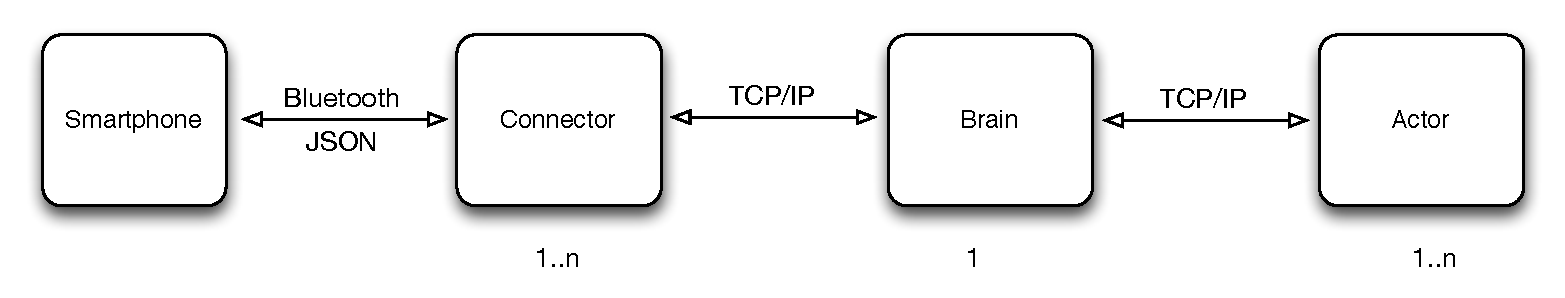
\includegraphics[width=12.5cm]{images/architecture}
\caption{Teilkomponenten und deren Relationen}
\end{figure}

Am offensichtlichsten ist die Anzahl der einzelnen Komponenten, welche innerhalb von InstantAmbient arbeiten. Des Weiteren Kommunizieren diese lediglich mit einem Vorgänger. Die Kette der Konfigurationsbereitstellung beginnt mit dem Smartphone bzw. der bereitgestellten App. Hier erstellt der User nach seinen individuellen Wünschen eine Konfiguration für unterschiedlichste Umgebungen. Soll diese beispielsweise vor der Fahrt mit einem Mietwagen übertragen werden, verbindet sich der Client mit dem Connector\footnote{In Zukunft auch InstantConnector genannt.}, wird die Konfiguration mit Hilfe von Bluetooth übertragen. Eine genauere Erläuterung der Technikauswahl ist in den nächsten Abschnitten zu finden. Der Connector an sich ist nur dafür zuständig die Daten entgegenzunehmen und diese zu validieren. Die eigentliche Prozessierung und Verteilung der Konfiguration findet im "`Brain"'\footnote{Zugegeben ist die Namenswahl ein wenig mutig, aber der Großteil der Backend-Logik befindet sich in diesem Modul.} statt. Für diesen Zweck überträgt der Connector die empfangene und validierte Konfiguration via TCP/IP zum Brain. Dieses unterhält mit Hilfe verschiedenen Mechanismen ein Verständnis welche Teile einer Konfigurationen zum Actor verschickt werden müssen. Hierbei wurde sich dafür entschieden, dass Aktoren immer für eine bestimmte Sektion der Konfiguration zuständig sind. Daher routet das Brain Sektionen zu einzelnen Aktoren. Es kann durchaus sein, dass ein Actor nur bestimmte Dateiformate unterstützt, daher ist im Brain eine Konvertierung beispielsweise von JSON zu XML vorgesehen.
Als letzte Komponente stehen die Aktoren, welcher vom Brain die konvertierte Sektion wieder via TCP/IP empfängt und verarbeitet. Verschiedenste Dienste können als Actor gesehen werden, sei es die Steuerung, der Heizung, der Multimediaanlage oder Sicherheitssysteme im Auto.
\\\\
Auf den ersten Blick scheint die hohe Anzahl der einzelnen Komponenten vielleicht für etwas übertrieben, aber gerade diese Entscheidung bürgt wesentliche Vorteile. Jede einzelne Komponente ist um ein leichtes austauschbar, besonders trifft dies auf den Connector und Actor zu. Gerade bei den Aktoren ist es nahezu logisch, da es eine Vielzahl an anzusprechenden Systemen und Protokollen gibt. Des Weiteren ist die derzeitige Entscheidung für Bluetooth keine feste, sondern können mit wenig Aufwand weitere Connectoren genutzt werden. Mehr Details dazu sind im Kapitel über das Backend zu finden. Bis auf das Brain kann bzw. muss jede weitere Komponente mehrmals existieren, genau dieser Fakt ist eine grundlegende Prämisse für skalierende konfigurationsbasierte Systeme. 
\\\\
Die folgenden Abschnitte, werden die Komponenten genauer erläutern.

\section{Aufbau Client}

Wie Bereits im Überblick angesprochen, wurde bei der Umsetzung für den Client eine Androide-App entwickelt. Diese muss dem Benutzer ein leichten einstieg in die Anwendung geben, daher sind die Wege zum in der App kurz gehalten. Näheres dazu folgt im Kapitel über den Client. 
Des Weiteren ist es so, dass der Client als Datenspeicher dient um die einbestellen Konfigurationen zu speichern. Hier bei wurde auf die in Android enthaltene SQLite Datenbank zurückgegriffen. 
Neben dem speichern der Daten und dem Bereitstellen einer Benutzerschnittstelle für den User, generiert der Client aus den Konfigurationsdaten eine JSON Objekt. Dieses wird nach dem Aufbau einer Bluetoothverbindung an den Connector gesendet. 
Dies geschieht alles im Hintergrund, da der User so wenig wie möglich davon mitbekommen soll. Dabei müssen allerdings verschiedene Aspekte betrachtet werden, wodurch folgende Fragen entstehen: Wann soll der Client die Daten Übertragen? Wann soll der Client eine neue Umgebung anlegen? Soll der Client eine Umgebung selbstständig anlegen. 
\\\\
Es ist natürlich am Benutzerfreundlichsten für den User wenn er so wenig wie möglich selber machen muss, ohne das die Anwendung in bevormundet. 
Daher ist es so, dass man beim initialen Start der Anwendung seine Allgemeine Konfiguration eingeben kann. 
Der Client erkennt automatisch wenn er sich in einer neuen Umgebung befindet. Nun kann der User für seine Umgebung, die beim erstmaligen anlegen für das Hotel oder Auto allgemein gültig ist, eine Konfiguration anlegen. 
Besucht der Benutzer zu einem späteren Zeitpunkt das gleiche Hotel, so wird beim betreten des Raumes und öffnen des Clients
die Konfiguration automatisch übertragen. 

\section{Aufbau Backend}
Wie bereits im Überblick erläutert, besteht das Backend aus mehreren untereinander austauschbaren Komponenten. Die Vorteile wurden bereits diskutiert, jedoch müssen eben diese drei Komponenten konzipiert und untereinander verbunden werden.
Im folgenden wird näher auf die Komponenten eingegangen ohne auf die spezifische Implementierung einzugehen.

\subsection{Connector}
Die Vorgänge innerhalb des Connectors sind unspektakulär. Bewusst soll diese Komponente einfach und leichtgewichtig gehalten werden. Mit Hilfe von Bluetooth, genauer gesagt dem Protokoll SPP, kann der Client seine serialisierte Konfiguration übertragen. Als erster Bearbeitungsschritt wird die Validität der Daten geprüft. Korrupte Dateien sollen so früh wie möglich aussortiert werden um die Sicherheit des Systems zu gewährleisten. In der Übersicht zur Gesamtübersicht wurde bewusst ein weiterer Bearbeitungsschritt nicht genannt. In vielen Fällen möchte das Brain eventuell wissen von welchem Connector die Daten kommen. Dies gilt besonders bei Szenarien wie etwa Hotels, Konfigurationen müssen eindeutig einer Umgebung zugeordnet sein. Daher modifiziert der Connector als zweiten Schritt die Konfiguration und fügt spezifische Informationen zur Umgebung zu. In den meisten Fällen reicht eine ID zur Identifikation. Als letzter Schritt wird das Brain mit der modifizierten Konfiguration kontaktiert und die Daten gesendet. 

\subsection{Brain}

Das Brain empfängt die valide Konfiguration mit Hilfe von TCP/IP. Nahezu jedes Systems stellt diese Schnittstellen bereit, viele Systeme und Architekturen basieren auf diese Kommunikationsmittel.
Die Hauptaufgabe des Brain liegt im Routing der Konfiguration. Hier stellen sich zwei wesentliche Fragen: Wie werden welche Daten geroutet, welche Formate besitzen diese? Und wie wird das Routing selbst abgebildet und konfiguriert? 
\\\\
Wie bereits angesprochen wird bei dem Routing angenommen, dass bestimmte Aktoren für einzelne Sektionen zuständig sind. Das heisst, dass ein Aktor die Teilkonfiguration beispielsweise für das Badezimmer empfängt. Dabei können mehrere Aktoren die Teilkonfiguration empfangen. Da in vielen Szenarien davon ausgegangen werden muss, dass nicht jeder Actor JSON spricht, sollte vor dem Senden der Daten eine mögliche Konvertierung stattfinden. Anfangs wird ebenfalls angenommen, dass die Aktoren über eine TCP/IP-Schnittstelle verfügen. 
\\\\
Des Weiteren ist die wohl größte Herausforderung auf einer eleganten Art und Weise das Routing darzustellen. Hierfür eignen sich entweder weitere Konfigurationsdateien, welche schnell unübersichtlich werden können oder auch domainspezifische Sprachen. Um ein wenig vorweg zugreifen wurde im Proof of Concept sich für die zweite Alternative entschieden. Das Routing muss im wesentlichen Kenntnisse über zwei Aspekte haben: 

\begin{enumerate}
     \item Der Definition von erreichbaren Aktoren
     \item Der Beschreibung welche Sektionen zu den einzelnen Aktoren gehören
   \end{enumerate}
\\\\
Besonders das Routing kann sehr schnell eine komplexe Aufgaben werden. Die Lösung ist im 8. Kapitel zu finden.

\subsection{Actor}
Ähnlich wie der Connector handelt es sich um den Actor um einer leichtgewichtige Komponente in Anbetracht der Kommunikation mit dem Brain. Die Systeme welche letztendlich damit gesteuert werden wie Heimautomatisierungsanlagen, haben zudem zusätzlich einen weiteren Grad an Komplexität. 
Im Grunde empfängt der Actor einen validen und eventuell konvertierten Teil der Konfiguration und spricht damit seine angebundenen Systeme an. Diese Komponente muss schmal und leichtgewichtig sein um die Austauschbarkeit zu garantieren.

\subsection{Mögliche Erweiterungen}
Die vorgestellte Architektur ist kein starres Konstrukt, sondern auch dafür vorgesehen erweitert zu werden. So sind eine Vielzahl an weiteren Services denkbar, wie beispielsweise die Integration von Authentifizierungs- oder Webservices. 

\begin{figure}[H]
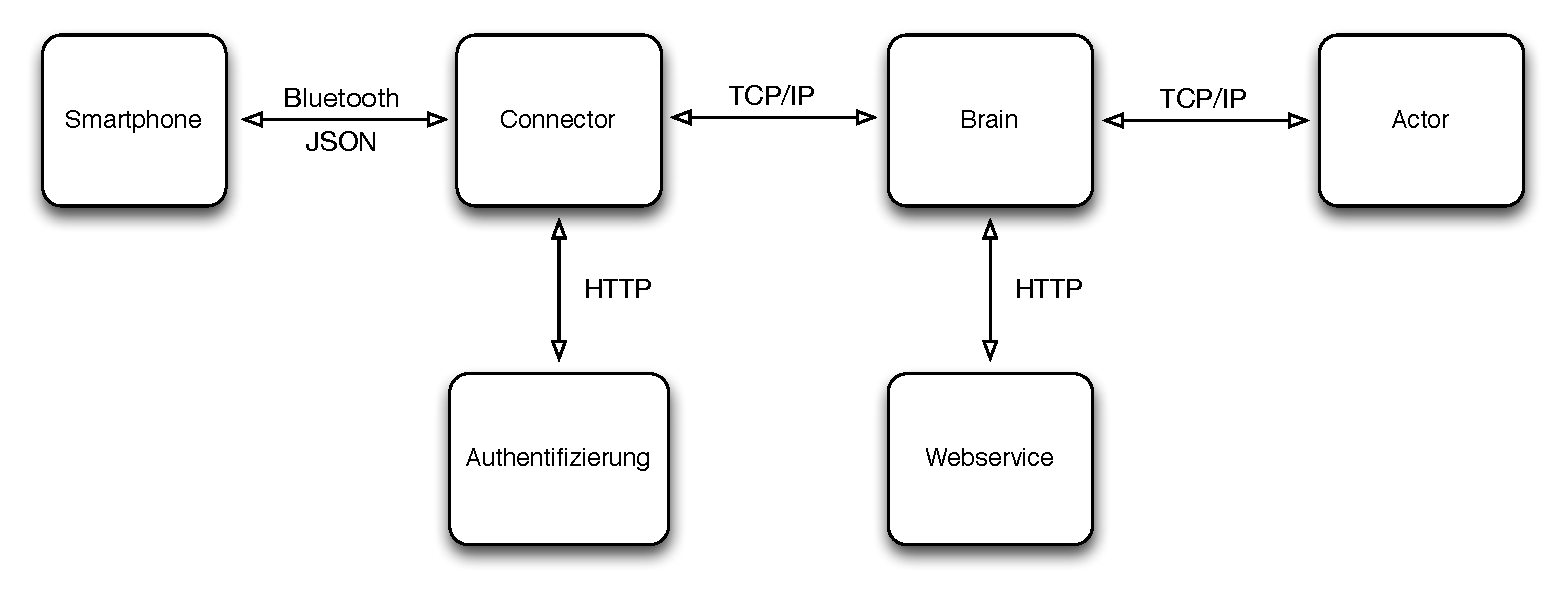
\includegraphics[width=12.5cm]{images/extended_architecture}
\caption{Erweiterte Architektur mit Web- und Authentifizierungsservice}
\end{figure}

Da z.B. bei der Authentifizierung nur das Brain als wesentliche Instanz mit den Service kommunizieren muss, steigt die Komplexität nur in diesem Teil der Anwendung. Damit soll gezeigt werden, dass die Wahl mehrere Teilsysteme zu nutzen den Vorteil hat, das System einfach zu erweitern und die Bedürfnisse einzelner Szenarien anzupassen. 

\section{Technologien}
Die Auswahl der Technologien richtet sich zum großen Teil an die Anwendungsszenarien und vorherrschende Architektur. So sollte die Auswahl der eingesetzten Programmiersprachen und Frameworks erst nach der Konzeption vorgenommen werden, anstatt bereits zu Projektbeginn. Dieser Abschnitt widmet sich der Auswahl der Technologien aller Komponenten und diskutiert verschiedenste Möglichkeiten des Einsatzes. 

\subsection{Client}
Wie bereits öfter angeschnitten, handelt es sich bei dem Client um eine auf Android basierende Smartphone-App. Daher verfällt die Wahl der Programmiersprache und es kommt Java mit dem Android SDK der Version 10 (Android 2.3.3) zum Einsatz. Für die Generierung der serialisierten Konfigurationen wurde das interne JSON-Framework eingesetzt. Um zusätzlich einen Eindruck über die UI gewinnen zu können, wurde das MockUp-Tool Balsamiq eingesetzt.
Die Wahl auf Android erfolgte auf Grund zweier Hauptkriterien: 

\begin{enumerate}
     \item Android selbst ist ein offenes System und kann auf eine große Community bauen. Des Weiteren ist der Bluetooth Support besonders in der Version 2.1 gegeben. 
     \item Innerhalb der Projektgruppe, gab es schon großes Know-How für diese Platform
\end{enumerate}
\\\\
Generell ist die Entwicklung für jede andere Smartphone-Platform möglich, solange diese Bluetooth unterstützt. Die von Apple vertriebenen Produkte und im besonderen das iPhone, unterstützen derzeit lediglich den neusten Bluetooth 4.0 Standard, für denen es wenige Implementierungen gibt, auch im Hinblick auf den Connector. 


\subsection{NFC}
Die Entscheidung auf Bluetooth wurde in dieser Dokumentation einfach als gegeben gesehen. Dennoch gibt es eine Vielzahl an Gründen warum sich für diese Art der Kommunikation entschieden wurde. 
Zunächst soll der Begriff NFC genauer beleuchtet werden. Im genaueren Technologischen Sinne, handelt es sich um eine Reihe von Standards unter anderem auch RFID, welche die Kommunikation zwischen verschiedensten NFC fähigen Endgeräten ermöglicht. Im weiteren Sinne beschreibt der Ausdruck NFC lediglich die Möglichkeit der Kommunikation verschiedenster Geräte in einem engeren Radius. Darunter kann WiFi, Bluetooth oder auch der XBee-Standard fallen. Die folgende Tabelle soll die Vorteile von Bluetooth gegenüber NFC aufzeigen: 

  \begin{table}
     \centering
     \begin{tabular}{| l | c | c |}
			\hline
      \textbf{Eigenschaften} & \textbf{NFC}  & \textbf{Bluetooth} \\ \hline
       Bandbreite  & -	& + \\ \hline
       Platformen  & Android, Nokia & iOS, Android, Blackberry...   \\ \hline
       Verbreitung & + & +   \\ \hline
			 Sicherheit  & + & + \\ \hline
			 Implementierung  & - & + \\ \hline
			
     \end{tabular} 
 
     \caption{Vergleich zwischen NFC und Bluetooth }
 
   \end{table}

\\\\
Neben den in der Tabelle aufgezeigten Vorteilen, bringen derzeitige NFC-Implementierungen mit sich. Die Größe der übertragenen Nachrichten müssen einer bestimmten Größe entsprechen, bei libnfc beträgt diese 53 Byte. Dies reicht unter Umständen für kleinere Konfigurationen aus, wenn aber auch Listen von TV-Sendern etc. mitgeschickt werden und UTF-16 codiert sind, werden diese Grenzen schnell gesprengt. 
Wie in der Architekturbeschreibung bereits angemerkt, ist die hier getroffene Wahl kein Dogma für das komplette Projekt, sondern der Connector kann durch seine leichtgewichtige Konzeption jederzeit ohne Probleme ausgetauscht werden.


\subsection{Connector}

Der Connector dient als Schnittstelle zwischen dem Client und Brain, daher ist dessen Hauptaufgabe die Übermittlung und Validierung empfangener Konfigurationen. Die Anzahl der frei verfügbaren und besonders Plattformunabhängigen Bluetooth-Implementierungen ist rar. Lediglich die in Java implementierte und spärlich gepflegte Bluecove-Library konnte den Anforderungen genügen. Der Vorteil an der Java-Platform ist ebenfalls, dass per se auch andere Sprachen eingesetzt werden können. In diesem Hinblick wurde sich für Ruby und der auf der JVM basierenden JRuby Implementierung entschieden. Ruby bietet den Vorteil eine moderne, elegante Sprache zu sein, welche insbesondere dafür geeignet ist in Szenarien wie InstantAmbient und dem Proof of Concept eingesetzt zu werden.
\\\\
Die Kommunikation zum Brain basiert auf einfachen TCP-Sockets, da diese ebenfalls auf jedem System verfügbar und die einfachste Variante der Datenübertragung sind. Eine weitere Alternative wäre der Einsatz von Messaging-Systemen wie AMQP oder ZeroMQ zu nutzen, welches jedoch für die erste Version einen enormen Overhead bedeutet hätte.


\subsection{Brain}

Das Brain bildet die zentrale Instanz des Backends. Es empfängt sämtliche Daten der Connectors, bearbeitet leitet diese an die entsprechenden Actoren. Hierfür müssen unter Umständen eine Vielzahl von gleichzeitigen Netzwerkverbindungen etabliert werden. Dieses Szenario lässt sich mit dem ebenfalls für Ruby entwickelten Framework Eventmachine abbilden. Es wurde dafür konzipiert eine große Anzahl an gleichzeitigen I/Os zu verarbeiten ohne das ganze System zu blockieren. Dieses Konzept wird ebenfalls unter anderem in Twisted für Python oder Node.js für Javascript genutzt. Besonders im Brain kann Ruby seine stärken ausspielen, da die Beschreibung des Routings in einer Domänspezifischen Sprache abgebildet wird. Des Weiteren kommen Bilbiotheken im Umgang mit JSON, XML hinzu. Die Actors werden ebenfalls via TCP/IP kontaktiert. 

\subsection{Actor} 
Wie im Falle des Connectors, ist der Actor selbst eher schmal gehalten. Dieser empfäng ebenfalls via Eventmachine die relevanten und konvertierten Teile der Konfiguration und schickt diese Informationen an die anschließenden Systeme. Bei der Beispielimplementierung wird hierfür ein Arduino eingesetzt. 
\\\\
Die genauen Details zur Implementierung und Umsetzung des Proof of Concepts sind in den nächsten zwei Kapitel ausführlich dokumentiert. 






